% !TEX program = xelatex
\documentclass[a4paper,nobib]{tufte-handout}

\usepackage{fontspec}
\usepackage{booktabs}
\usepackage{tabularx}
\usepackage{graphicx}
\usepackage{amsmath}
\usepackage{xcolor}
\usepackage{listings}
\usepackage{xurl}

\setmainfont{Palatino}
\setsansfont{Helvetica}
\setmonofont{Menlo}
\emergencystretch=2em
\graphicspath{{../results/figures/}}
\definecolor{codebg}{HTML}{F4F5F6}
\lstset{basicstyle=\ttfamily\footnotesize,backgroundcolor=\color{codebg},
  breaklines=true,columns=fullflexible,showstringspaces=false,
  xleftmargin=0.5em,xrightmargin=0.5em,aboveskip=0.6em,belowskip=0.7em}

\title[Lab 1 Report]{Lab 1: Linux, Shell, and C++ Foundations}
\author{Xuanye Xu (24020036071 / H00490299)}
\date{24 September 2026}

\begin{document}
\maketitle
\pagestyle{fancy}
\fancyhf{}
\fancyfoot[C]{\small\thepage}
\renewcommand{\headrulewidth}{0pt}
\thispagestyle{fancy}

\begin{abstract}
This report documents all five assessed parts of Lab 1. An official Ubuntu
20.04.6 LTS x86\_64 image was installed as a WSL 2 distribution on a Windows
host and configured for command-line C++ development. Direct \texttt{g++} and
CMake builds succeeded. Shell exercises produced reproducible text counts and
a file containing five appended \texttt{fortune} results. Ten C++ warm-up
answers were checked with a compiled program. Finally, the supplied
\texttt{RandomVector} interface was implemented and tested, including
histogram conservation and boundary cases. Each assessed part below identifies
its method, observed result, and saved evidence.
\end{abstract}

\begin{fullwidth}
\small
\begin{tabularx}{\linewidth}{@{}p{0.42in}p{1.95in}p{0.7in}X@{}}
\toprule
No. & Assessed part & Points & Primary evidence \\
\midrule
1 & Ubuntu installation and setup & 40 & Distribution, architecture, account, and tool versions (Fig.~\ref{fig:ubuntu}); real terminal-window screenshot (Fig.~\ref{fig:ubuntu-window}). \\
2 & Compile example code & 5 & Successful \texttt{g++} and CMake builds and executable output (Fig.~\ref{fig:compile}). \\
3 & Shell operations & 5 & Dante counts and five appended fortunes (Fig.~\ref{fig:shell}). \\
4 & C++ questions & 25 & Ten reasoned answers and compiled checks (Fig.~\ref{fig:warmup}). \\
5 & C++ practice & 25 & Implemented class, histogram, and boundary checks (Fig.~\ref{fig:vector}). \\
\bottomrule
\end{tabularx}
\end{fullwidth}

\section{1. Ubuntu installation and setup (40 points)}

The course slide requests Ubuntu 20.04 and recommends a virtual machine for
classroom use. For this experiment I used an x86\_64 Windows host running
\textbf{WSL 2}, with a separate \texttt{Ubuntu-20.04} distribution. The existing
Ubuntu 26.04 distribution was left in place. It is not a bare-metal
installation and has no separate Ubuntu desktop session; Linux GUI programs
are shown directly on the Windows desktop through WSLg
(Figure~\ref{fig:ubuntu-window}). Lab~2 later ran turtlesim and RViz in the
same way; the Unity simulators of Labs~3 and~4 have not been tested yet.

The official Ubuntu 20.04.6 WSL image was downloaded from the Ubuntu release
site. Its SHA-256 was checked against the published \texttt{SHA256SUMS}; the
full matching digest is recorded in \texttt{results/environment.txt}.
The Windows \texttt{wsl.exe --list --verbose} output identified
\texttt{Ubuntu-20.04} as version 2. Within that distribution,
\texttt{/etc/os-release} identified Ubuntu 20.04.6 LTS and \texttt{uname -m}
reported \texttt{x86\_64}. The normal user \texttt{qz} has \texttt{sudo}
membership and a working password, entered by the owner during first-run
setup.

After updating and upgrading the package lists, I installed
\path{build-essential}, CMake, and Git. The measured versions were
\texttt{g++ 9.4.0}, \texttt{cmake 3.16.3}, \texttt{git 2.25.1}, and
\texttt{GNU Make 4.2.1}. A C++ compiler smoke test built without warnings and
printed \texttt{Ubuntu 20.04 toolchain OK}. Figure~\ref{fig:ubuntu} shows a
fresh verification of the OS, architecture, user, and packages.
Figure~\ref{fig:ubuntu-window} is a real screenshot of an Ubuntu terminal
window (xterm) opened through WSLg, in which the same checks were typed; its
transcript is saved beside the image.

\begin{figure*}[!htbp]
\centering
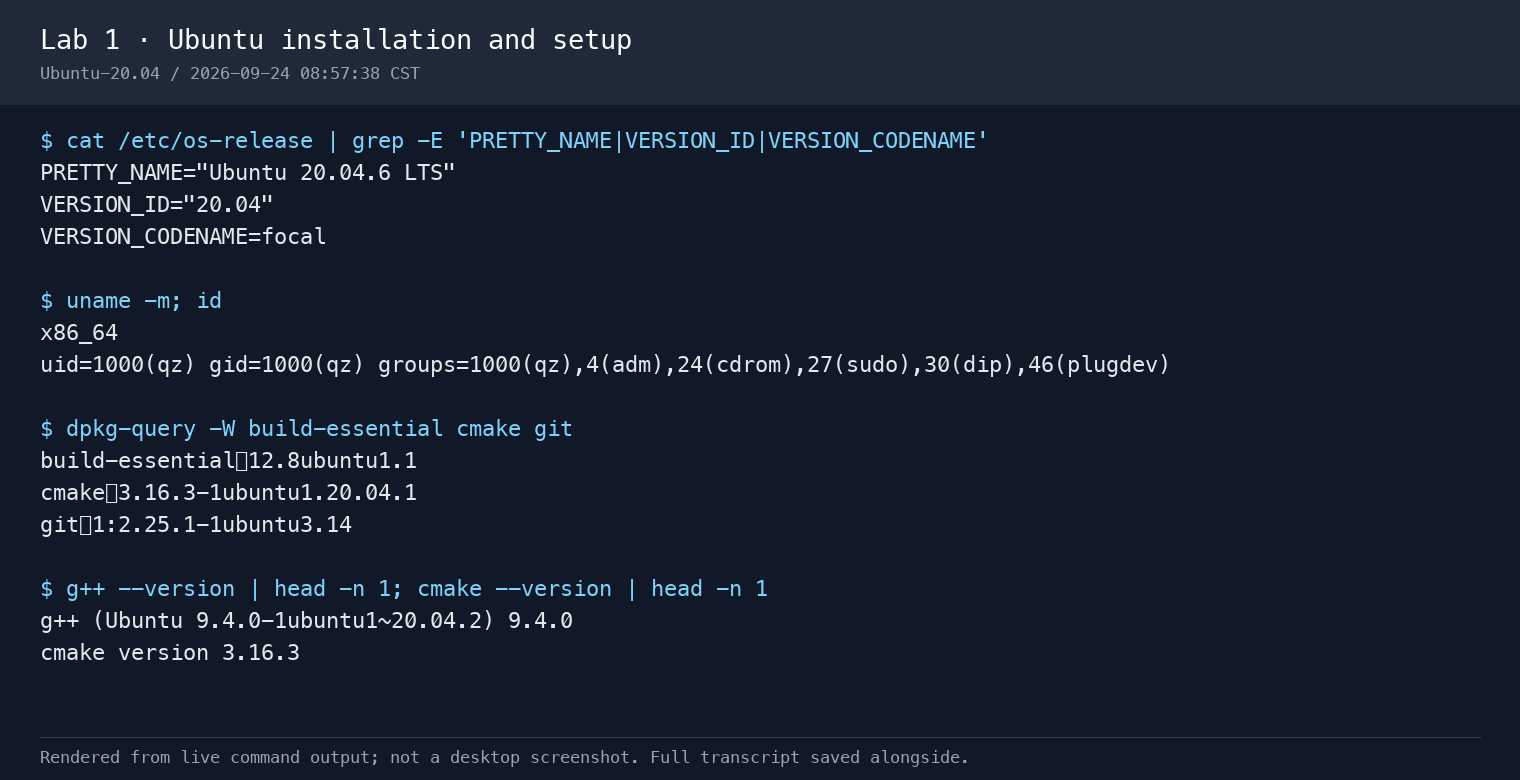
\includegraphics[width=\linewidth]{01_ubuntu_environment.png}
\caption{Ubuntu environment verification. This figure is typeset from live
SSH/WSL command output and retains its original text transcript; it is not a
desktop-window screenshot.\protect\label{fig:ubuntu}}
\end{figure*}

\begin{figure*}[!htbp]
\centering
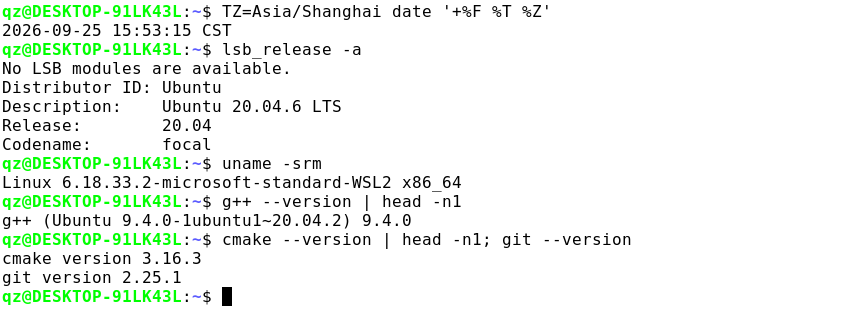
\includegraphics[width=0.8\linewidth]{01b_ubuntu_terminal_window.png}
\caption{Real screenshot of an Ubuntu 20.04 terminal window (xterm) displayed
on the Windows desktop through WSLg, 25 September 2026. The commands were
typed into this interactive shell and the window was captured from the X
server; transcript in
\texttt{results/\allowbreak figures/\allowbreak 01b\_\allowbreak ubuntu\_\allowbreak terminal\_\allowbreak window.txt}.\protect\label{fig:ubuntu-window}}
\end{figure*}
\FloatBarrier

\section{2. Compiling example code (5 points)}

I compiled a single-file example with C++11, warnings, and pedantic checking:
\begin{lstlisting}
g++ -std=c++11 -Wall -Wextra -pedantic hello.cpp -o hello
./hello
\end{lstlisting}
The executable printed ``Hello from Lab 1 on Ubuntu 20.04!''. I then
configured and built a multi-file CMake example. Its \texttt{message.cpp}
was compiled into a static library, and \texttt{main.cpp} linked against that
library. The final executable printed \texttt{CMake library link OK}. Both
build routes exited with status 0 and produced no compiler diagnostics.
This contrast made the distinction between compiling source files and linking
an executable concrete.

\begin{figure*}[!htbp]
\centering
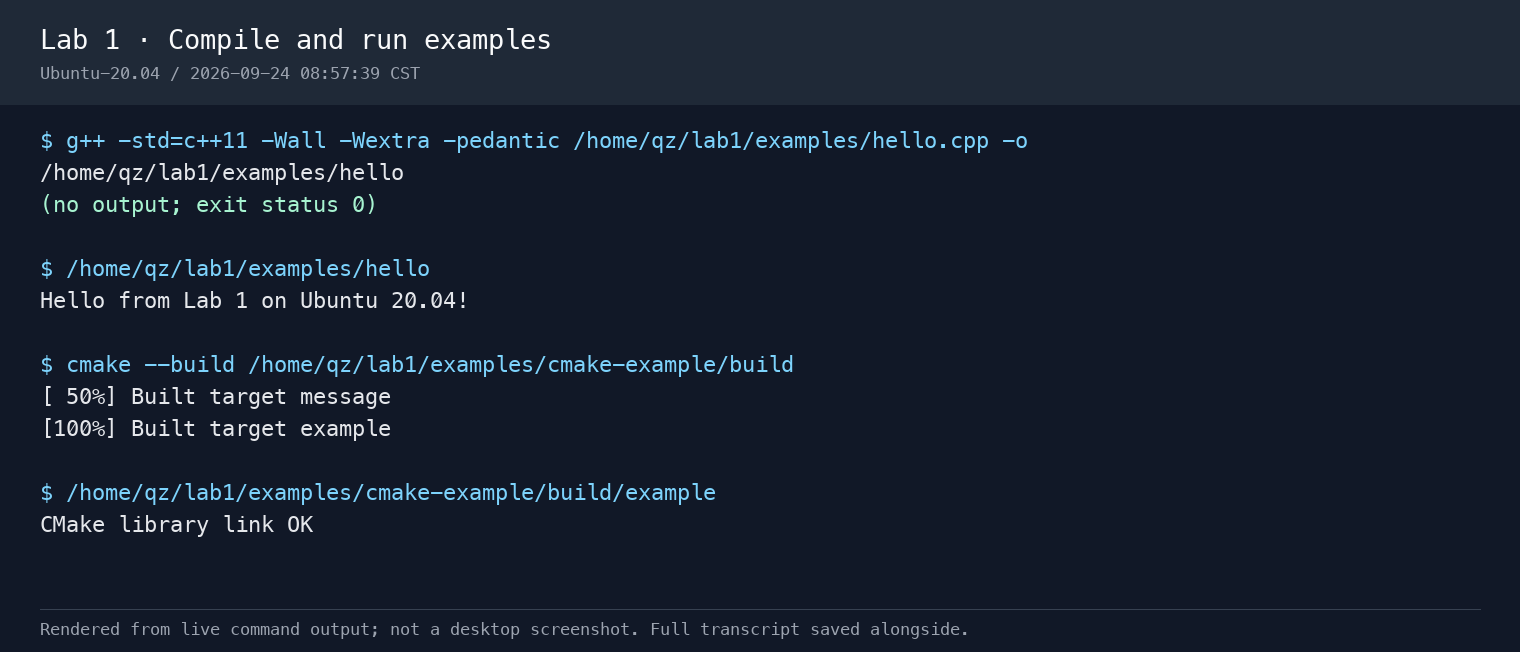
\includegraphics[width=\linewidth]{02_compile_examples.png}
\caption{Direct C++ compilation and CMake build, followed by the two actual
program outputs. Rendered from live SSH/WSL output.\protect\label{fig:compile}}
\end{figure*}
\FloatBarrier

\section{3. Shell operations (5 points)}

For the text-counting exercise, the \texttt{dante.txt} file was obtained from
the repository named in the MIT exercise. The original direct download did
not complete in this network environment, so I used a CDN copy of the same
repository file and compared it byte-for-byte with the GitHub Contents API
response before counting. The saved input contains 557,042 bytes; its SHA-256
is recorded in \texttt{results/shell.txt}.

\begin{fullwidth}
\small
\begin{tabularx}{\linewidth}{@{}XrX@{}}
\toprule
Ubuntu command & Result & Interpretation \\
\midrule
\texttt{wc -l dante.txt} & 19,567 & Newline-terminated lines. \\
\texttt{wc -w dante.txt} & 97,676 & Words under the Ubuntu locale used for the exercise. \\
\texttt{grep -cve '\^{}[[:space:]]*\$' dante.txt} & 14,338 & Lines containing non-whitespace text. \\
\bottomrule
\end{tabularx}
\end{fullwidth}

For output redirection, a script created \texttt{fortunes.txt} once and
executed \texttt{/usr/games/fortune >> fortunes.txt} five times. The
cumulative byte totals after each append were 53, 175, 365, 388, and 441.
The final file is 441 bytes. Its nine text lines do not imply nine invocations:
a single fortune may span multiple lines. I also exercised \texttt{mkdir},
\texttt{cd}, \texttt{pwd}, copying, moving, \texttt{chmod}, \texttt{find}, pipes,
and \texttt{wc}. Figure~\ref{fig:shell} records the counts and the append
script. The original text and script remain available for inspection.

The word count differed under the default macOS locale (97,765) even though
the bytes were identical; \texttt{LC\_ALL=C} on macOS gave 97,676. Therefore
the submitted result is explicitly the value measured in Ubuntu, with the
command and environment stated.

\begin{figure*}[!htbp]
\centering
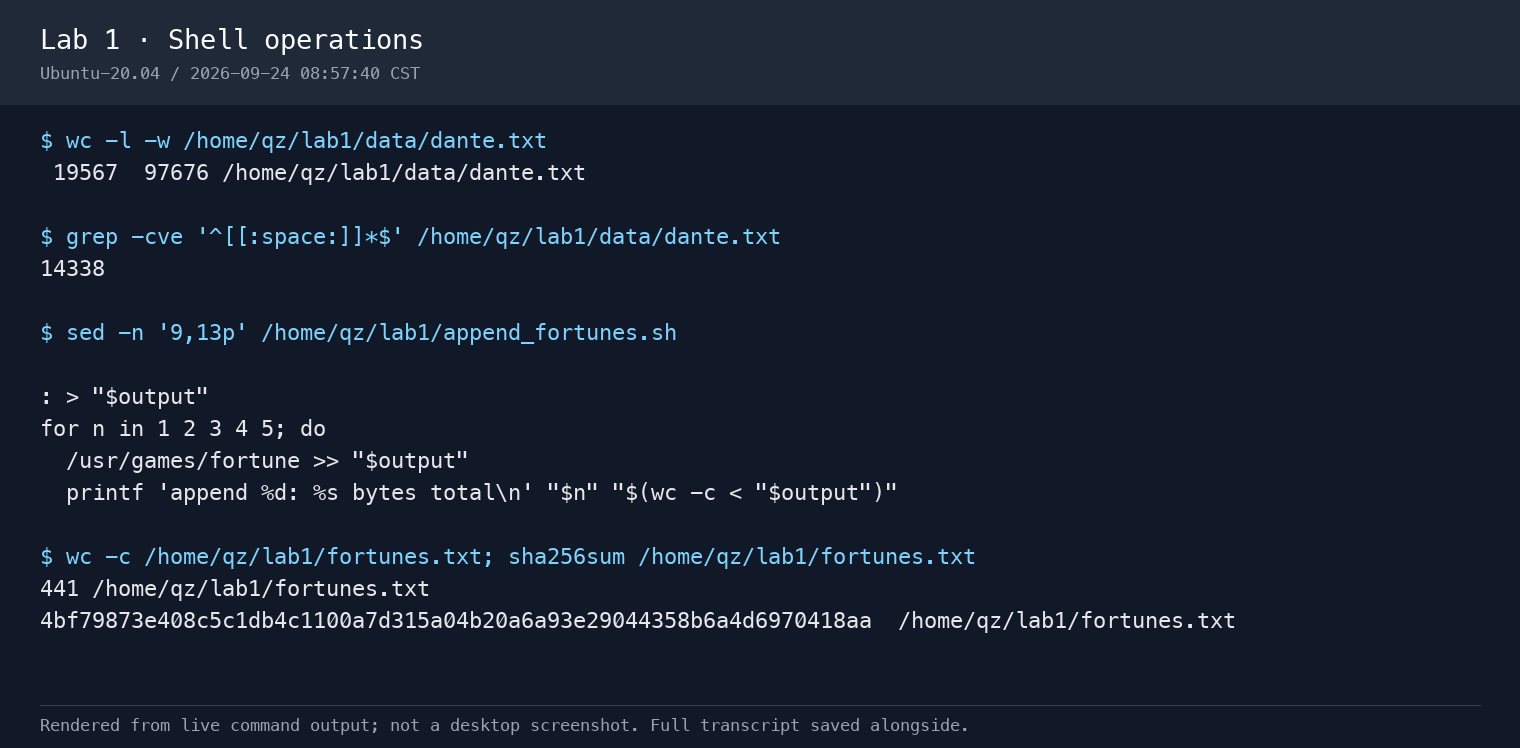
\includegraphics[width=\linewidth]{03_shell_operations.png}
\caption{Dante line/word counts, nonblank-line count, five-append script, and
final fortune-file size and hash. Rendered from live SSH/WSL output.\protect\label{fig:shell}}
\end{figure*}
\FloatBarrier

\section{4. C++ warm-up questions (25 points)}

I answered all ten questions in the order of the MIT warm-up exercise. The
short conclusions below are paired with the reasoning needed to explain them
at an experiment check. The complete answer file is
\texttt{lab1/cpp-warmup.txt}; \texttt{cpp\_warmup\_check.cpp} executes the
corresponding snippets.

\noindent\textbf{O1 --- Pre- and post-increment.} After \texttt{j = ++i;}
and then \texttt{j = i++;}, \(i=2\) and \(j=1\). The first assignment uses
the incremented value; the second assigns the old value before incrementing.

\noindent\textbf{O2 --- Conditional operator.} The expression
\texttt{42 < 42} is false, so the program prints \texttt{b}.

\noindent\textbf{R1 --- Reference alias.} The output is \texttt{10 10}.
The reference and original integer name the same object; writing through
the reference changes the original.

\noindent\textbf{R2 --- Pointer dereference.} The expression
\texttt{*j**j} parses as \texttt{(*j) * (*j)}, not exponentiation. It stores
\(42\times42=1764\) through the pointer and prints \texttt{1764}.

\noindent\textbf{R3 --- Pointer arithmetic.} \texttt{i + 2} addresses the
third array element. The assignment uses the second and fourth elements,
\(24-24=0\), so the program prints \texttt{0}.

\noindent\textbf{R4 --- Reference parameter.} The function's
\texttt{int\&} parameter aliases the caller's \texttt{j}. Resetting it to
zero makes the program print \texttt{0}.

\noindent\textbf{N1 --- Integer types.} \texttt{short}, \texttt{int},
\texttt{long}, and \texttt{long long} have nondecreasing required ranges,
but byte widths depend on the ABI. On this Ubuntu x86\_64 installation,
\texttt{sizeof} measured 2, 4, 8, and 8 bytes respectively. These are
measurements, not portable constants.

\noindent\textbf{N2 --- Floating-point and conversion.} \texttt{double}
provides at least the precision/range of \texttt{float}; here they occupy 8
and 4 bytes respectively. Assigning the \texttt{double} literal \texttt{3.14}
to an \texttt{int} discards the fractional part, so \(i=3\).

\noindent\textbf{N3 --- Unsigned conversion.} With 8-bit
\texttt{unsigned char}, converting \(-1\) is modulo 256, so \(c=255\).
The assumption about character width is essential.

\noindent\textbf{N4 --- Boolean condition.} Nonzero \texttt{42} converts
to true. The first branch sets \(i=0\); the \texttt{else} branch is skipped.

The compiled run in Figure~\ref{fig:warmup} agreed with every predicted
value. The source file and plain-text output are kept alongside the report.

\begin{figure*}[!htbp]
\centering
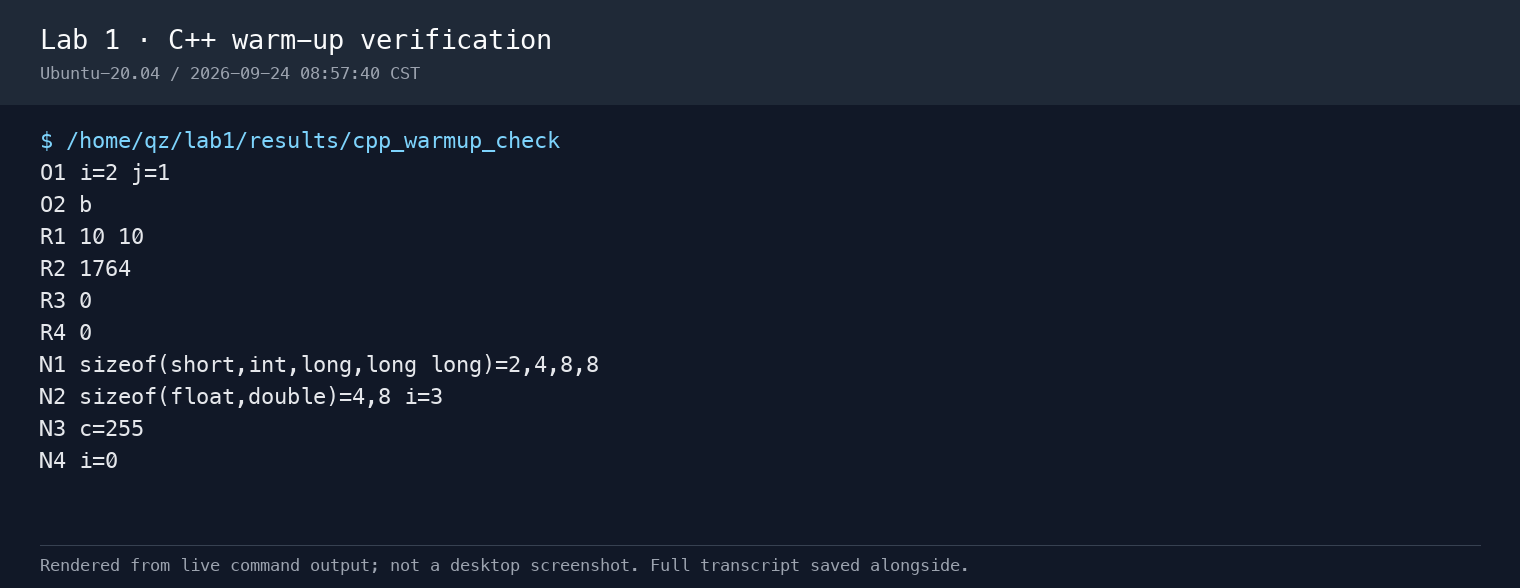
\includegraphics[width=\linewidth]{04_cpp_warmup.png}
\caption{Compiled verification of all ten C++ warm-up answers, including
platform-specific type sizes. Rendered from live SSH/WSL output.\protect\label{fig:warmup}}
\end{figure*}
\FloatBarrier

\section{5. C++ practice: RandomVector (25 points)}

I kept the original MIT class interface and demonstration entry point and
filled the six methods in \texttt{random\_vector.cpp}. The constructor
generates \texttt{size} doubles by scaling \texttt{std::rand()} with a
floating-point divisor, avoiding integer truncation:
\[
  x_i = \frac{\operatorname{rand}()} {\mathrm{RAND\_MAX}}\,\texttt{max\_val},
  \qquad 0\leq x_i\leq\texttt{max\_val}.
\]
The demonstration seeds the generator with 314159. The \texttt{print} method
emits every value; \texttt{mean}, \texttt{min}, and \texttt{max} use simple
loops and no functions from \texttt{<algorithm>}.

For \(B\) histogram bins between observed minimum \(m\) and maximum \(M\),
the index is
\[
  b(x)=\min\!\left(\left\lfloor B\frac{x-m}{M-m}\right\rfloor,
  B-1\right),\qquad M>m.
\]
Thus regular bins are left-closed and right-open, while the last bin includes
the maximum. For \(M=m\), all values go into the first bin to avoid division
by zero. The histogram is printed as vertical columns. Invalid size,
nonfinite or negative upper bound, and nonpositive bin count raise
\texttt{std::invalid\_argument}.

The Ubuntu default run produced 20 values with mean \(0.55804\), minimum
\(0.0278694\), and maximum \(0.982655\). Its five column counts were
\(5,1,4,3,7\), summing exactly to 20. Figure~\ref{fig:vector} shows both the
actual histogram and the verification summary. The test program also checked
the printed value count and range, independent bin classification from the
seeded inputs, a singleton, zero and scaled upper bounds, one bin, more bins
than values, and invalid arguments. All passed on Ubuntu 20.04.

The Ubuntu sequence differs from the MIT sample and a local macOS run. A
fixed seed reproduces the sequence within one \texttt{std::rand()}
implementation, but the C library does not promise the same sequence across
platforms. The requirements are therefore checked by range, statistics, and
bin conservation rather than by copying the sample numbers.

\begin{figure*}[!htbp]
\centering
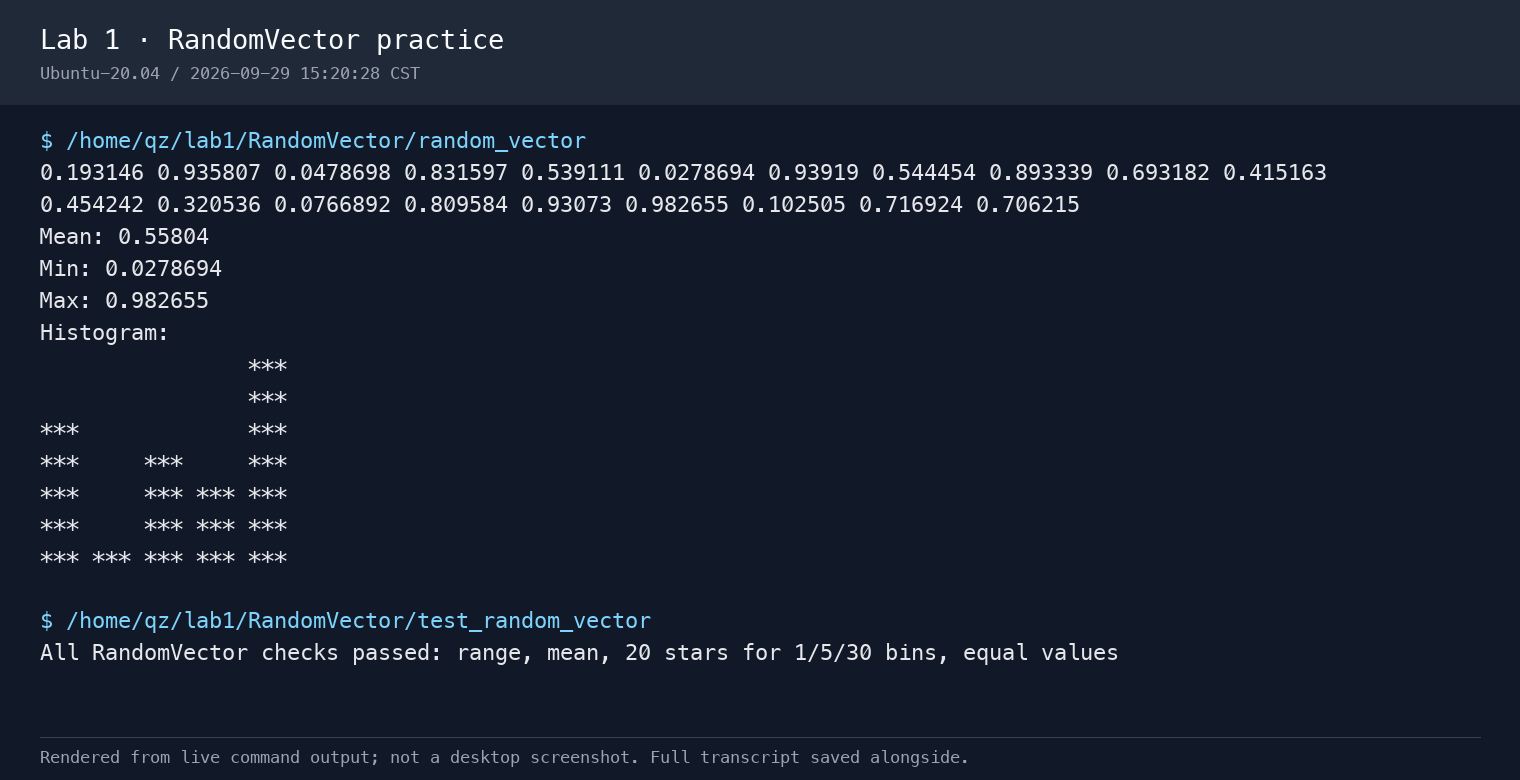
\includegraphics[width=\linewidth]{05_random_vector.png}
\caption{\texttt{RandomVector} default output and boundary verification on
Ubuntu 20.04. Rendered from live SSH/WSL output.\protect\label{fig:vector}}
\end{figure*}
\FloatBarrier

\section{Discussion and reproducibility}

The two cross-platform discrepancies were instructive. The same Dante bytes
gave different default word counts on macOS and Ubuntu because the counting
locale differed. The same C++ random seed gave different values because
\texttt{std::rand()} implementations differed. Both cases show why an
experimental result needs its command, environment, and input, not just its
final number. The histogram required an explicit upper-bound rule: without
clamping the maximum to the last bin, the natural formula can index past the
array. These were verified with the original inputs and targeted boundary
checks rather than inferred from the example output.

WSL 2 supported all Lab 1 command-line tasks, and WSLg displays Linux GUI
windows (Figure~\ref{fig:ubuntu-window}). The Unity simulators of later labs
still need their own validation.

To reproduce the C++ practice from \texttt{lab1/RandomVector} on Ubuntu:
\begin{lstlisting}
g++ -std=c++11 -Wall -Wextra -pedantic \
  main.cpp random_vector.cpp -o random_vector
./random_vector
g++ -std=c++11 -Wall -Wextra -pedantic \
  test_random_vector.cpp random_vector.cpp \
  -o test_random_vector
./test_random_vector
\end{lstlisting}
The answer file, source code, and command transcripts accompany this PDF in
the Lab 1 directory. Each figure renders saved live SSH/WSL output with an
adjacent text transcript; it is not a native window screenshot.

\section{References}
\begin{fullwidth}
\footnotesize
\begin{enumerate}
\item Course materials, \emph{Lab 1} slides and \emph{Course Syllabus}, supplied in this project.
\item MIT VNAV, \emph{Lab 1 Exercises}, \url{https://vnav.mit.edu/labs_2023/lab1/exercises.html}.
\item MIT-SPARK, \emph{VNAV-labs Lab 1 source template}, \url{https://github.com/MIT-SPARK/VNAV-labs/tree/master/lab1}.
\item Ubuntu, \emph{Ubuntu 20.04.6 WSL image and SHA256SUMS}, \url{https://releases.ubuntu.com/focal/}.
\end{enumerate}
\end{fullwidth}

\end{document}
